\section{Theorie}
\label{sec:theorie}
%
Befindet sich ein Atom in einem gleichförmigen äußeren Magnetfeld, so spalten sich dessen Energieniveaus auf.
Dieses Phänomen wird als Zeeman-Effekt bezeichnet.
Experimentell lässt sich die Verschiebung über die Aufspaltung und Polarisation der durch die Atome emittierten Spektrallinien untersuchen.
Über sogenannte \enquote{Auswahlregeln} lassen sich in der Theorie Vorhersagen über die Energie und Polarisation der emittierten Strahlung machen.
%
\subsection{Drehimpuls und magnetisches Moment eines Elektrons}
%
Jedes Hüllenelektron besitzt zwei Drehimpulse, den Bahndrehimpuls~$\vec{l}$ und den Spin~$\vec{s}$.
Die Lösungen der quantenmechanischen Eigenwertgleichungen liefern für die Beträge der Drehimpulse
%
\begin{align}
    \lvert\,\vec{l}\,\rvert&=\sqrt{l(l+1)}\,\hbar\quad\text{mit}\quad l=0,1,2,\ldots,n-1
    \shortintertext{und}
    \lvert\,\vec{s}\,\rvert&=\sqrt{s(s+1)}\,\hbar\quad\text{mit}\quad s=\frac{1}{2}.
\end{align}
%
Die Drehimpulse bedingen je ein magnetisches Moment. Der Bahndrehimpuls liefert
%
\begin{gather}
    \vec{\mu}_l=-\mu_{\mathup{B}}\sqrt{l(l+1)}\,\vec{l}_0
    \intertext{mit dem Bohrschen Magneton}
    \mu_{\mathup{B}}:=-\frac{e_0\hbar}{2m_0}.
\end{gather}
%
Der Spin liefert
%
\begin{equation}
    \vec{\mu}_s=-g_s\sqrt{s(s+1)}\,\vec{s}_0
\end{equation}
%
mit dem Landé-Faktor~$g_s$ des Elektrons, der in etwa den Wert~$2$ hat.
Für den Zustand mit $s=\sfrac{1}{2}$ und $l=1$ ist $\vec{\mu}_s$ ungefähr doppelt so groß wie $\vec{\mu}_l$.
Dieser Umstand wird auch als magnetomechanische Anomalie des Elektrons bezeichnet.
Der exakte Wert von~$g_s$ ergibt sich aus der relativistischen Theorie des Elektrons nach Dirac.
%
\subsection{Wechselwirkungen der Drehimpulse und der magnetischen Momente}
%
Im Folgenden werden die Wechselwirkungen der Drehimpulse eines Mehrelektronenatoms betrachtet.
Die beiden Drehimpulse eines Elektrons wechselwirken sowohl untereinander, als auch mit den Drehimpulsen anderer Elektronen in der Hülle.
Da diese Überlagerung der Wechselwirkungen in der Theorie schwer zu beschreiben ist, werden zwei Grenzfälle betrachtet:

\textbf{1. Grenzfall:}
Bei Atomen mit niedriger Kernladungszahl ist die Wechselwirkung zwischen den Bahndrehimpulsen verschiedener Elektronen so groß, dass sich diese zum Gesamtbahndrehimpuls~$\vec{L}$ addieren, wobei
%
\begin{align}
    \lvert\,\vec{L}\,\rvert&=\sqrt{L(L+1)}\,\hbar\quad\text{mit}\quad L=0,1,2,\ldots
    \intertext{gilt. Gemäß der gebräuchlichen Notation in der Atomphysik werden die verschiedenen Werte von $L$ aufsteigend mit den Buchstaben $S,P,D,F,\ldots$ gekennzeichnet. Analog zu den Bahndrehimpulsen kombinieren sich auch die Spins der Elektronen additiv zum Gesamtspin~$\vec{S}$. Es gilt}
    \lvert\,\vec{S}\,\rvert&=\sqrt{S(S+1)}\,\hbar\quad\text{mit}\quad S=\frac{N}{2},\frac{N}{2}-1,\ldots,\frac{1}{2},0
\end{align}
%
wobei $N$ die Anzahl der Hüllenelektronen ist.
Auch dem Gesamtbahndrehimpuls~$\vec{L}$ und dem Gesamtspin~$\vec{S}$ wird mit
%
\begin{align}
    \lvert\,\vec{\mu}_L\,\rvert&=\mu_{\mathup{B}}\sqrt{L(L+1)}
    \shortintertext{und}
    \lvert\,\vec{\mu}_S\,\rvert&=g_S\mu_{\mathup{B}}\sqrt{S(S+1)}
\end{align}
%
ein magnetisches Moment zugeordnet.
Für nicht zu starke Magnetfelder ergibt sich ein Gesamtdrehimpuls
%
\begin{gather}
    \vec{J}=\vec{L}+\vec{S}
    \shortintertext{mit}
    \lvert\,\vec{J}\,\rvert=\sqrt{J(J+1)}
\end{gather}
%
wobei $J$ entweder ganz- oder halbzahlig sein kann.
Der obige Zusammenhang wird auch als $LS$-Kopplung oder Russell-Saunders-Kopplung bezeichnet.
$J$ wird üblicherweise als unterer Index an den Symbolen $S,P,D,F,\ldots$ notiert.
Oberer Index ist die Multiplizität~$M=2S+1$.

\textbf{2. Grenzfall:}
Bei schweren Atomen ist die Wechselwirkung zwischen Spin und Bahndrehimpuls eines Elektrons groß gegenüber der Wechselwirkung der Bahndrehimpulse und Spins verschiedener Elektronen untereinander.
Es ergibt sich der Gesamtdrehimpuls
%
\begin{equation}
    \vec{j}_i=\vec{l}_i+\vec{s}_i
\end{equation}
%
je Einzelektron, sodass kein Gesamtdrehimpuls~$\vec{L}$ und Gesamtspin~$\vec{S}$ mehr definiert sind.
Die $\vec{j}_i$ addieren sich nun zum Gesamtdrehimpuls~$\vec{J}$.
Diese Art der Wechselwirkung wird auch als $j$-$j$-Kopplung bezeichnet.

Zwischen den genannten Grenzfällen existiert für mittlere Kernladungszahlen ein fließender Übergang.
%
\subsection{Aufspaltung der Energieniveaus eines Atoms im homogenen Magnetfeld}
%
Das zu $\vec{J}$ gehörende magnetische Moment ergibt sich zu
%
\begin{equation}
    \vec{\mu}=\vec{\mu}_L+\vec{\mu}_S.
\end{equation}
%
$\vec{J}$ und $\vec{\mu}$ sind im Allgemeinen nicht parallel, doch der Erwartungswert der zu $\vec{J}$ senkrechten Komponente verschwindet aufgrund der präzedierenden Bewegung um die Magnetfeldrichtung im zeitlichen Mittel.
Aus der Quantenmechanik folgt
%
\begin{equation}
     \lvert\,\vec{\mu}_J\,\rvert=g_J\mu_{\mathup{B}}\sqrt{J(J+1)}
\end{equation}
%
mit dem Landé-Faktor
%
\begin{equation}
    g_J:=\frac{3J(J+1)+S(S+1)-L(L+1)}{2J(J+1)}.
    \label{eq:g_J}
\end{equation}
%
Ein weiteres Resultat der Quantenmechanik ist die Richtungsquantelung im homogenen Magnetfeld.
Es gilt
%
\begin{equation}
    \mu_{J_z}=-mg_J\mu_{\mathup{B}}
\end{equation}
%
mit der Orientierungsquantenzahl $m\in\{-J,-J+1,\ldots,J-1,J\}$.
Daraus folgen $2J+1$ Einstellmöglichkeiten für ein magnetisches Moment in einem äußeren Magnetfeld.
Für die Energie, die ein Moment $\vec{\mu}$ im Magnetfeld erhält, ergibt sich
%
\begin{equation}
    E_{\mathup{mag}}=-\vec{\mu}\vec{B}=mg_J\mu_{\mathup{B}}B.
    \label{eq:E_mag}
\end{equation}
%
Das Energieniveau $E_0$ im feldfreien Raum spaltet bei $B\neq0$ in $2J+1$ äquidistante Niveaus auf.
Beispielhaft ist dies in Abbildung~\ref{fig:aufspaltung} für ein Atom mit $J=2$ skizziert.
Die Aufspaltung ermöglicht neue Übergänge zwischen Energieniveaus und somit neue Spektrallinien.
Dieser Effekt wird als Zeeman-Effekt bezeichnet.
%
\begin{figure}
    \centering
    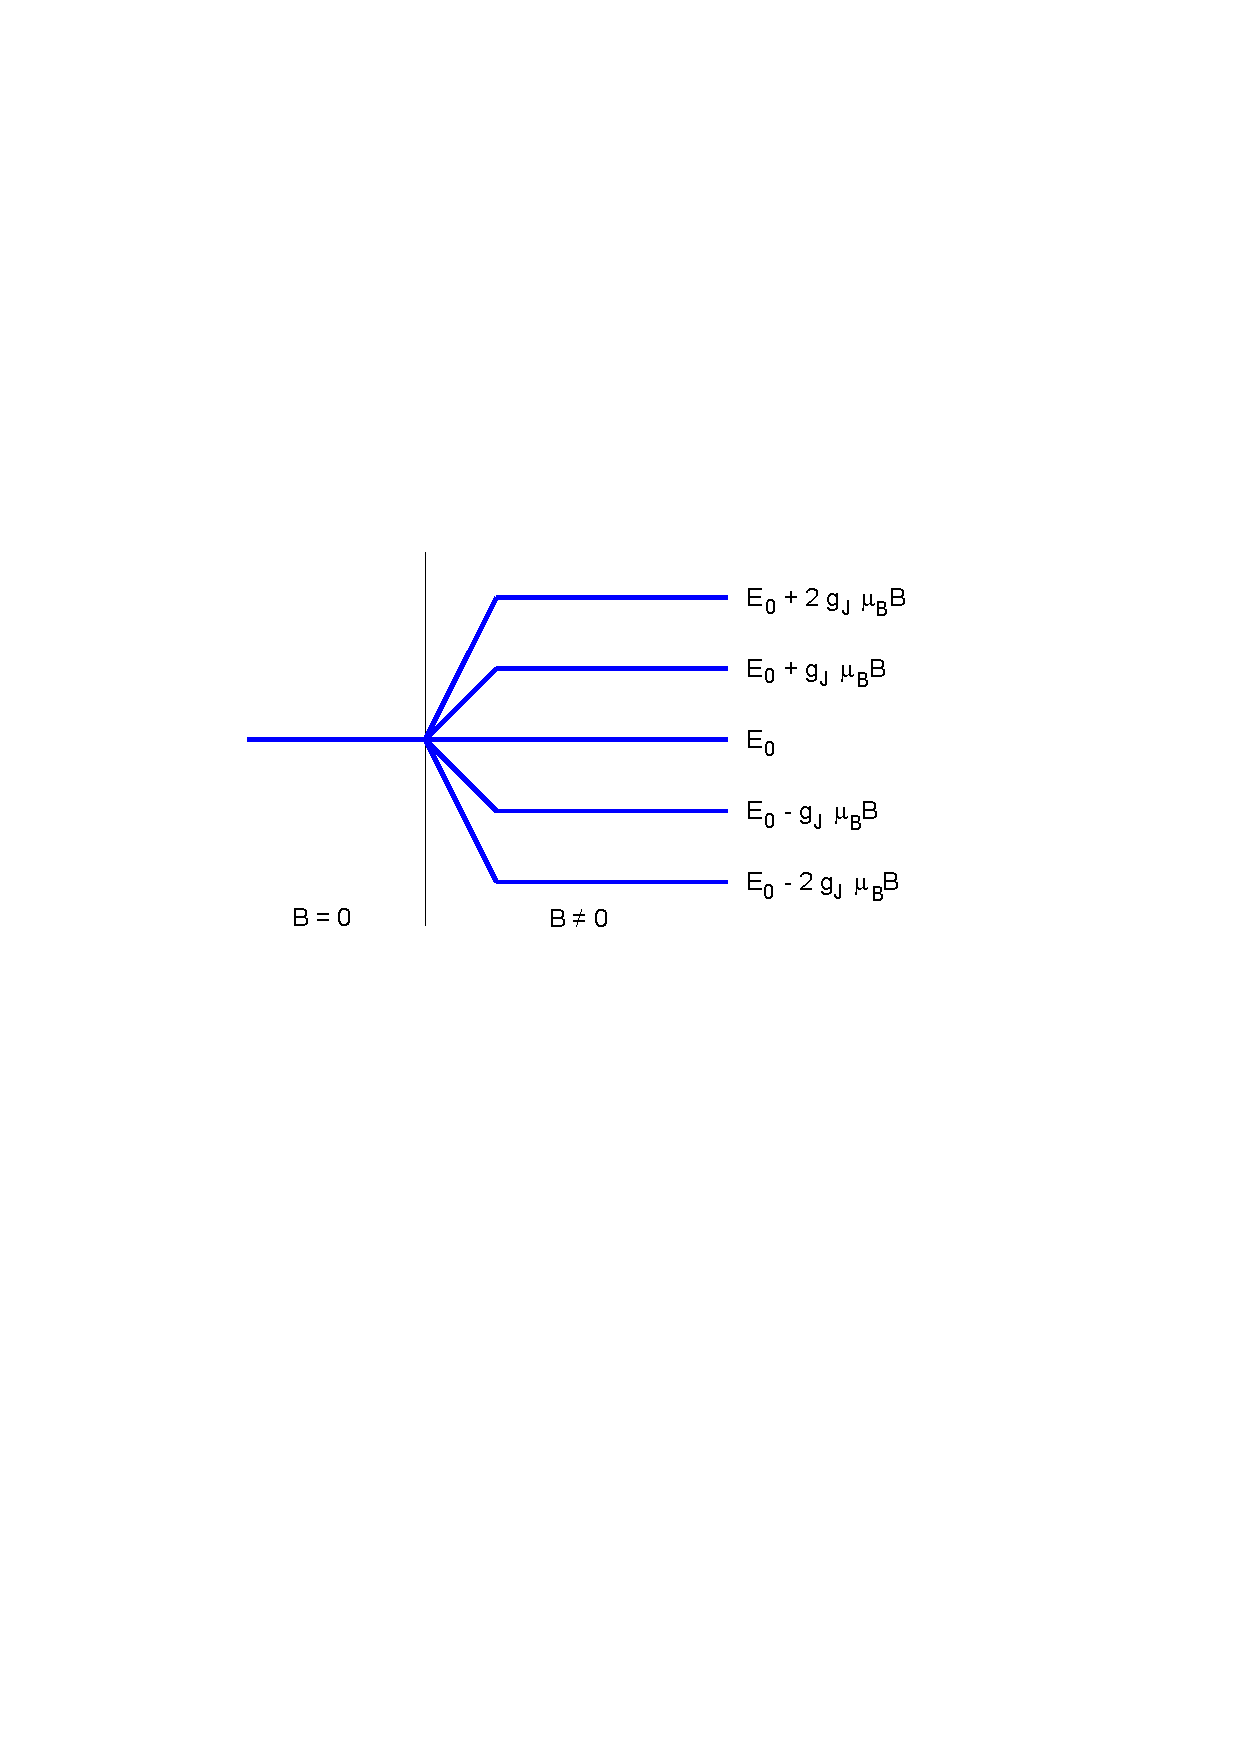
\includegraphics[width=0.6\textwidth]{figure/aufspaltung.pdf}
    \caption{Schematische Darstellung der Aufspaltung eines Energieniveaus eines Atoms mit Gesamtdrehimpulsquantenzahl $J=2$.\cite{V27}}
    \label{fig:aufspaltung}
\end{figure}
%
\subsection{Auswahlregeln für Übergänge zwischen aufgespaltenen Energieniveaus}
%
Im Folgenden wird die Herleitung der Auswahlregeln, die festlegen welche Übergänge zwischen verschiedenen Energieniveaus erlaubt sind, kurz skizziert.
Die Bestimmung der Auswahlregeln erfolgt durch die Betrachtung zweier möglicher Lösungen der zeitabhängigen Schrödingergleichung mit den zugehörigen Energien $E_{\alpha}$ und $E_{\beta}$.
Die Linearkombination beider Zustände liefert einen Zustand, der eine Schwingung des Elektrons mit der Frequenz
%
\begin{equation}
    \nu_{\alpha\beta}:=\frac{E_{\alpha}-E_{\beta}}{h}
\end{equation}
%
beschreibt.
Die Bestimmung der Intensität der emittierten Strahlung erfolgt über die Berechnung des elektrischen Dipolmomentes des Elektrons.
Eine längere Recnung ergibt, dass nur dann Spektrallinien emittiert werden, wenn sich die zu den Energien gehörigen Orientierungsquantenzahlen $m_{\alpha}$ und $m_{\beta}$ entweder garnicht oder um $\pm 1$ unterscheiden.
Weiterhin ergibt die Rechnung, dass ein Übergang mit $\upD m=0$ eine linear polarisierte und parallel zum Magnetfeld emittierte Strahlung liefert, wohingegen ein Übergang mit $\upD m=\pm1$ zu einer zirkular polarisierten Strahlung führt.
%
\subsection{Der Zeeman-Effekt}
%
\subsubsection{Der normale Zeeman-Effekt}
%
Alle (das wäre komisch) oben gemachten Erkenntnisse gelten zunächst nur für $S=0$, da der Spin in der zeitabhängigen Schrödingergleichung nicht auftaucht.
Daraus folgt mit Gleichung~\eqref{eq:g_J} immer $g_j=1$ unabhängig von $L$ und $J$.
Für die Energiedifferenz eines aufgespaltenen Niveaus ergibt sich aus Gleichung~\eqref{eq:E_mag}
%
\begin{equation}
    \upD E=\upD m\mu_{\mathup{B}}B
    \label{eq:dE_norm}
\end{equation}
%
mit $\upD m=m_1-m_2$. Die möglichen Übergänge führen zu drei Liniengruppen mit jeweils gleichem $\upD m$, dem sogenannten Zeeman-Triplett.
Abbildung~\ref{fig:zeeman_normal} zeigt die Aufspaltung und Übergänge für $J=2\rightarrow J=1$.
Die Linien mit $\upD m=0$ sind linear polarisiert und werden als $\pi$-Linien bezeichnet.
Sie sind nur mit voller Intensität zu sehen, wenn sie senkrecht zur Feldrichtung betrachtet werden.
Das heißt, dass das Aufspaltungsbild abhängig von der Beobachtungsrichtung ist.
Die zwei Liniengruppen mit $\upD m=\pm1$ werden als $\sigma$-Linien bezeichnet.
Die Liniengruppen selbst unterscheiden sich in ihrer Energie um jeweils den Wert $\mu_{\mathup{B}}B$ voneinander.
%
\begin{figure}
    \centering
    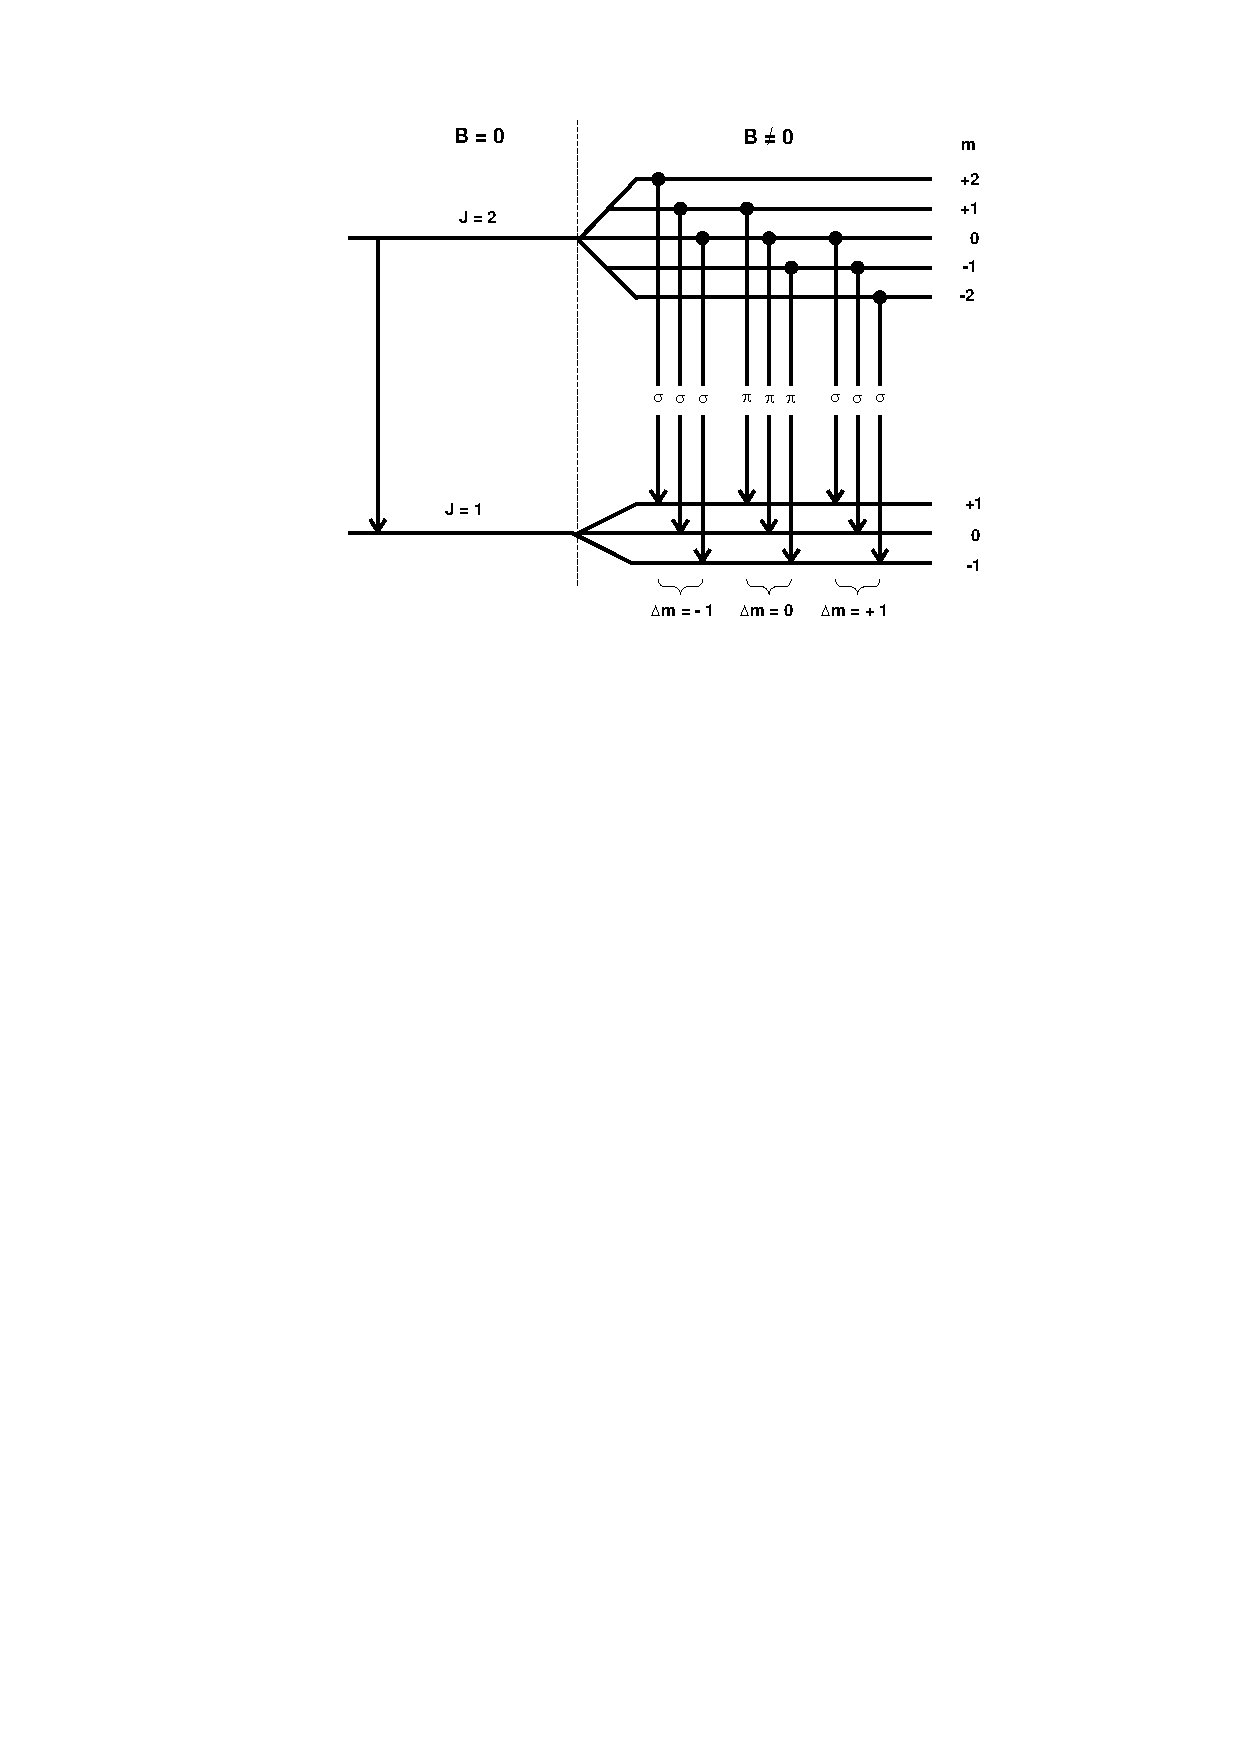
\includegraphics[width=0.65\textwidth]{figure/zeeman_normal.pdf}
    \caption{Beispiel einer Linienaufspaltung beim normalen Zeeman-Effekt.\cite{V27}}
    \label{fig:zeeman_normal}
\end{figure}
%
\subsubsection{Der anomale Zeeman-Effekt}
%
Der häufiger anzutreffende anomale Zeeman-Effekt beschreibt den Fall für $S\neq0$.
Die Herleitung der Auswahlregeln mit der spinabhängigen Schrödingergleichung liefert erstaunlicherweise dieselben Auswahlregeln wie in Abschnitt~\ref{sec:...}.
Für die Energiedifferenz ergibt sich nun
%
\begin{equation}
    \upD E=\left[m_1g(L_1,S_1,J_1)-m_2g(L_2,S_2,J_2)\right]\mu_{\mathup{B}}B.
    \label{eq:dE_ano}
\end{equation}
%
Hierbei entspricht der Term in den eckigen Klammern dem Landé-Faktor des Übergangs.
Abbildung~\ref{fig:zeeman_anomal} zeigt beispielhaft die Aufspaltung und Übergänge eines Alkali-Dubletts.
%
\begin{figure}
    \centering
    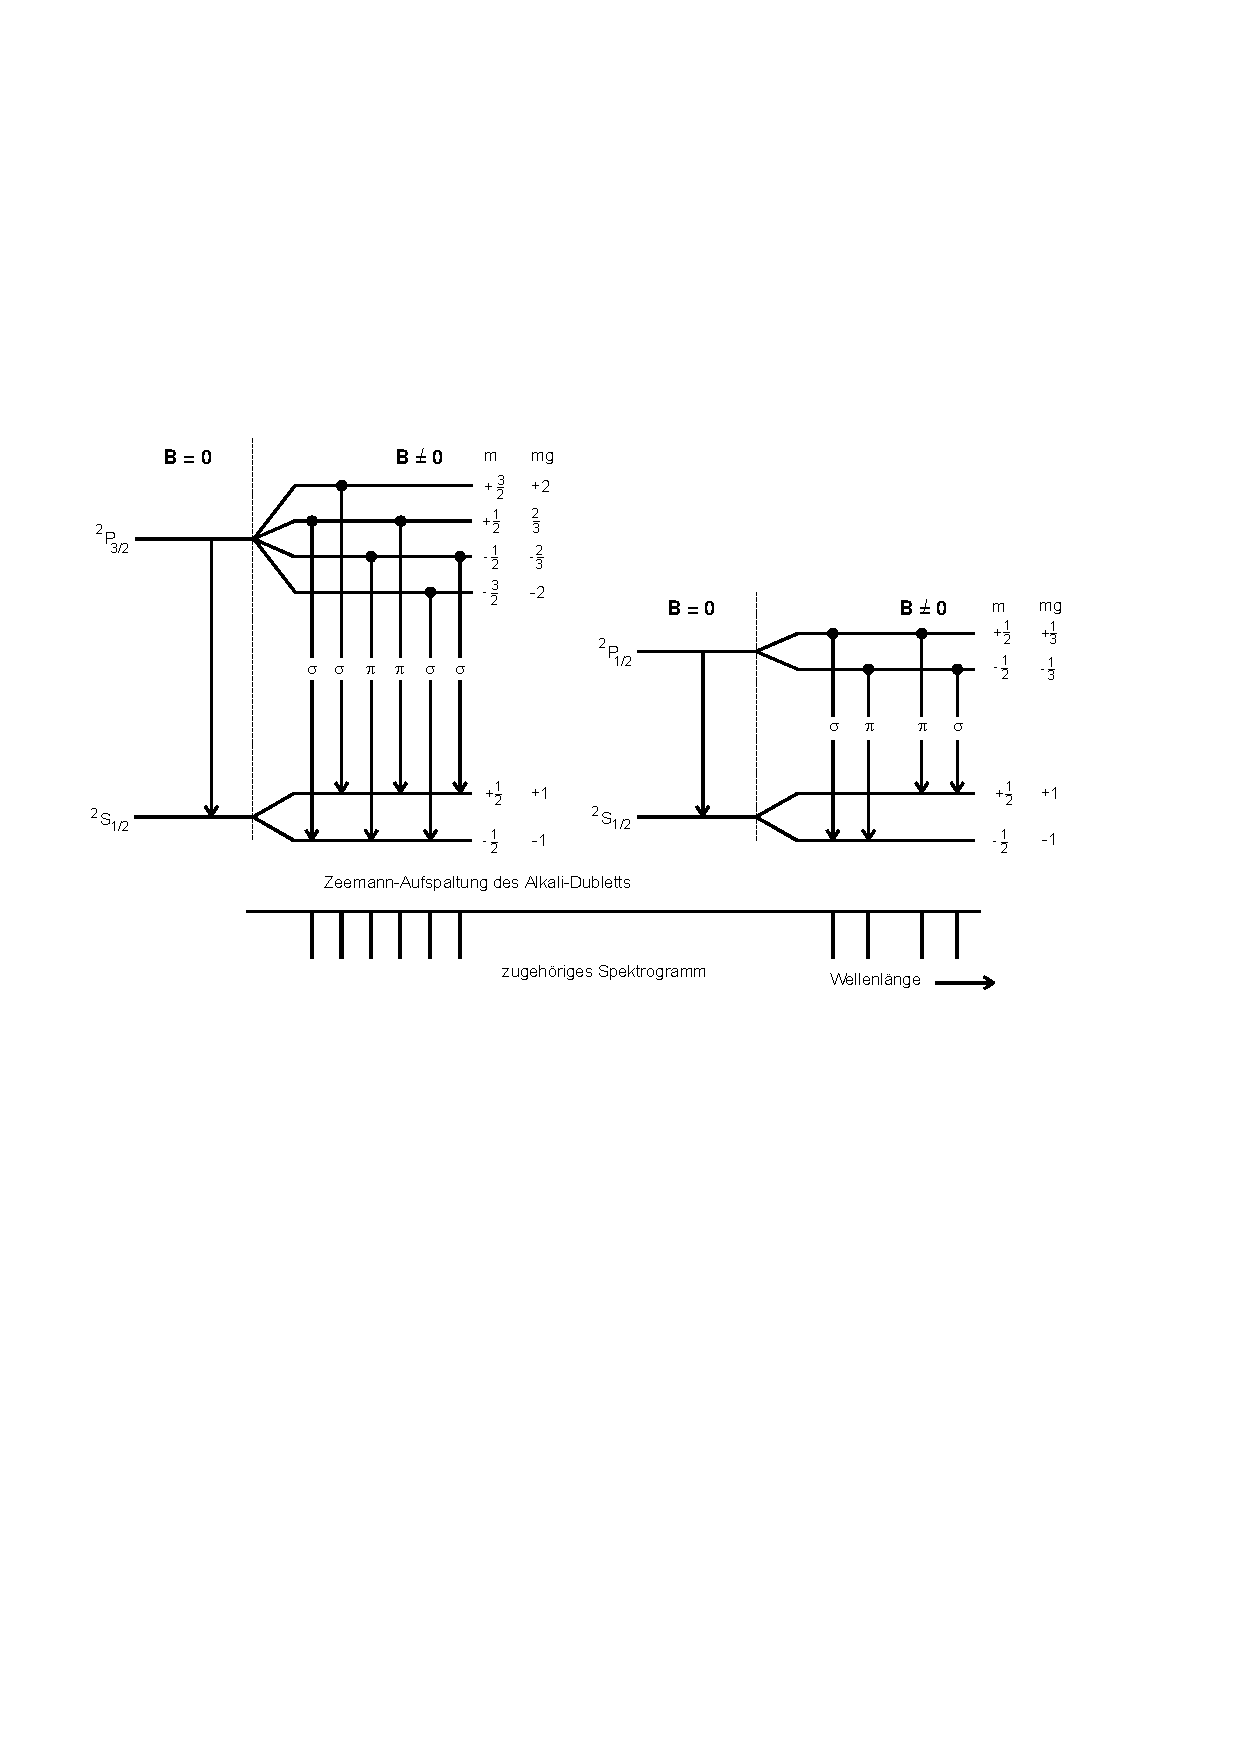
\includegraphics[width=\textwidth]{figure/zeeman_anomal.pdf}
    \caption{Beispiel einer Linienaufspaltung beim anomalen Zeeman-Effekt. Dargestellt ist die Aufspaltung eines Alkali-Dubletts.\cite{V27}}
    \label{fig:zeeman_anomal}
\end{figure}
